\section{Program Analysis}
\enumstart
	\item Can automatically learn facts about a program
	\\ 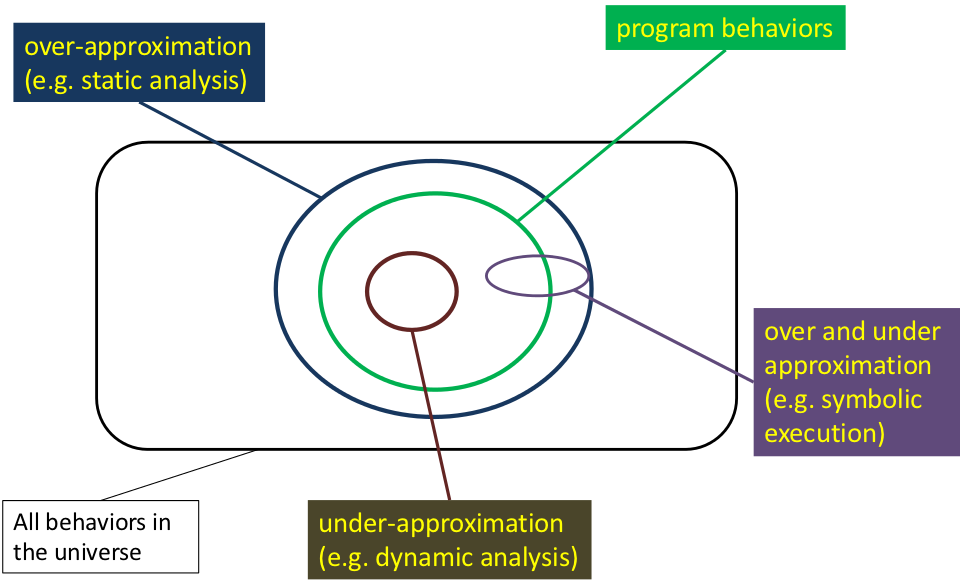
\includegraphics[width=0.5\textwidth]{img/program_analysis.png}
\enumend

\subsection{Static program analysis}
\enumstart
	\item We use abstract interpretation $\rightarrow$ a general theory of how to do approximation systematically
\enumend

\subsection{Abstract interpretation}
\enumstart
	\item Step-by-step
	\enumstart
		\item Select/define an abstract domain (depends on what you want to prove)
		\item Define abstract semantics for the language w.r.t. the domain
		\enumstart
			\item Prove sound w.r.t. concrete semantics
			\item Involves defining abstract transformers
		\enumend
		\item Iterate abstract transformers over the abstract domain $\rightarrow$ until fixpoint is reached
	\enumend
	\item The fixpoint is the over-approximation of the program
\enumend

\subsection{Abstract transformer}
\enumstart
	\item Effect of statement and expression evaluation on an abstract state
	\item Defined per programming language once and for all
	\item Abstract transformers define the abstract semantics of the language
	\item Correctness(soundness): produces a superset of what a concrete transformer would produce
	\item Precision: the set produced by the abstract transformer is as small as possible
	\item Goal, be perfectly sound and as precise as possible
	\item Sometimes, computing the most precise transformer (best transformer) is not possible
\enumend

\subsection{Iterate abstract transformers}
\enumstart
	\item Start with the least abstract element for all program-counter values
	\item Iterate the different statements/expressions and apply abstract transformers.
	\item Whenever we have two abstract elements $A$ and $B$, we can join them to produce their (least) upper bound (denoted by $A \sqcup B$)
	\item $A \sqsubseteq (A \sqcup B)$ and $B \sqsubseteq (A \sqcup B)$
	\item $D \sqsubseteq E$ means that $E$ is more abstract than $D$
	\item If it never terminates, do widening
\enumend

\subsection{Widening}
\enumstart
	\item Ensures termination at the expense of precision
	\item Do instead of join, whenever you like
\enumend

\subsection{Semantics}
\enumstart
	\item Why formal semantics?
	\enumstart
		\item Understand what a program does
		\item Implement a language
		\item Reasoning about program correctness
	\enumend
	\item Three approaches
	\enumstart
		\item Operational semantics
		\enumstart
			\item How would I execute the statement?
			\item Define a transition system, transition relation describes evaluation steps of a program
		\enumend
		\item Denotational semantics
		\enumstart
			\item What is the statement computing?
			\item Define an input/output relation that assigns meaning to each construct
		\enumend
		\item Axiomatic semantics
		\enumstart
			\item What is true after a statement is executed?
			\item Define the effect of each construct on logical statements about program store
		\enumend
	\enumend
\enumend

\subsection{SPL Language Syntax}
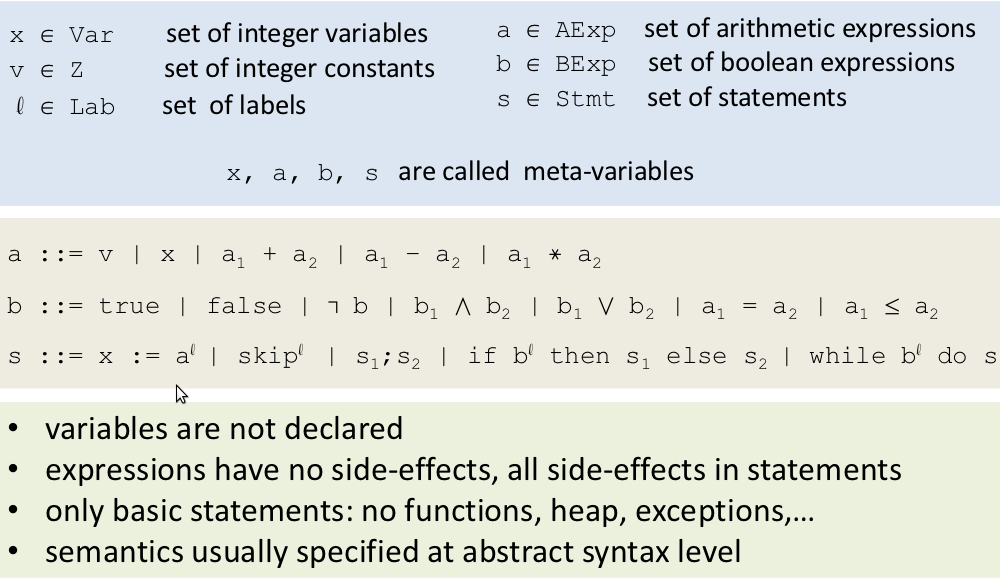
\includegraphics[width=0.5\textwidth]{img/spl_language_syntax.png}

\subsection{Operational semantics}
\enumstart
	\item Specifies how expressions and statements should be evaluated
	\item Evaluation depends on the shape of the expression/statement
	\item Evaluation depends on the values of variables
	\item Values of variables at any moment in time are given by a function $\sigma \in \text{Store} = \text{Var} \rightarrow Z$
	\item Configurations: $c \in \Sigma$ where $\Sigma = (\text{Stmt} \times \text{Store}) \cup \text{Store}$
	\enumstart
		\item $\la S, \sigma \ra$ is a configuration
		\item $\sigma$ is also a configuration, a terminal configuration
	\enumend
	\item Transitions: $\rightarrow \subseteq \Sigma \times \Sigma$ (steps between configurations)
	\item Transition system: $(\Sigma, \rightarrow, I, F)$
	\enumstart
		\item $I \subseteq \Sigma$: Initial configurations
		\item $F \subseteq \text{Store}$: final configurations
	\enumend
	\item $c \rightarrow c'$ denotes $(c, c') \in \rightarrow$
	\item $\rightarrow^*$ denotes the reflexive transitive closure of the relation $\rightarrow$
	\enumstart
		\item There is a sequence $c_0, \mathellipsis, c_n$ where $c_0 = c$, $c_n = c'$ and for all $0 \le i \le n-1$: $c_i \rightarrow c_{i+1}$
	\enumend
\enumend

\subsection{Operational semantics of SPL}

\subsubsection{Big-step semantics}
\enumstart
	\item We use it for arithmetic- and boolean expressions 
	\item $c \rightarrow c'$ describes the entire computation
	\item Some relations needed
	\enumstart
		\item $\Downarrow_a \subseteq (AExp \times Store) \times Z$
		\item $\Downarrow_b \subseteq (BExp \times Store) \times \{true, false\}$
		\item $\la a, \sigma \ra \Downarrow_a v$ means: "expression $a$ evaluates to $v$ in store $\sigma$"
	\enumend
	\item Evaluation rules for arithmetic expressions
	\enumstart
		\item $\frac{\la a_1, \sigma \ra \Downarrow_a v_1 \ \ \ \la a_2, \sigma \ra \Downarrow_a v_2}{\la a_1 + a_2, \sigma \ra \Downarrow_a v_1 + v_2}$
		\item $\frac{}{\la x, \sigma \ra \Downarrow_a \sigma(x)}$
	\enumend
	\item Evaluation rules for boolean expressions
	\enumstart
		\item $\frac{\la a_1, \sigma \ra \Downarrow_a v_1 \ \ \ \la a_2, \sigma \ra \Downarrow_a v_2}{\la a_1 \le a_2, \sigma \ra \Downarrow_b bv}$ bv is $v_1 \le v_2$
		\item $\frac{\la a_1, \sigma \ra \Downarrow_a v_1 \ \ \ \la a_2, \sigma \ra \Downarrow_a v_2}{\la a_1 = a_2, \sigma \ra \Downarrow_b bv}$ bv is $v_1 == v_2$
		\item $\frac{\la b_1, \sigma \ra \Downarrow_b true \ \ \ \la b_2, \sigma \ra \Downarrow_b true}{\la b_1 \land b_2, \sigma \ra \Downarrow_b true}$
		\item $\frac{\la b_1, \sigma \ra \Downarrow_b false}{\la b_1 \land b_2, \sigma \ra \Downarrow_b false}$
		\item $\frac{\la b_2, \sigma \ra \Downarrow_b false}{\la b_1 \land b_2, \sigma \ra \Downarrow_b false}$ adsf
	\enumend
\enumend

\subsubsection{Small-step semantics}
\enumstart
	\item We use it for statements
	\item $c \rightarrow c'$ describes a single step of a larger computation
	\item Evaluating a statement produces a new store ($\la s, \sigma \ra \rightarrow \la s', \sigma' \ra$)
	\item Evaluation order is important
	\enumstart
		\item In "$s_1;s_2$", $s_1$ is evaluated before $s_2$
		\item In "if true then $s_1$ else $s_2$", $s_2$ is not evaluated
	\enumend
	\item Evaluation rules for Stmt
	\enumstart
		\item $\frac{\la s_1, \sigma \ra \rightarrow \la s_2, \sigma_1 \ra}{\la s_1;s_3, \sigma \ra \rightarrow \la s_2;s_3, \sigma_1 \ra}$ bla
		\item $\frac{\la s_1, \sigma \ra \rightarrow \sigma_1}{\la s_1;s_2, \sigma \ra \rightarrow \la s_2, \sigma_1 \ra}$
		\item $\frac{}{\la skip, \sigma \ra \rightarrow \sigma}$
		\item $\frac{\la a, \sigma \ra \Downarrow_a v}{\la x := a, \sigma \ra \rightarrow \la x := v, \sigma \ra}$
		\item $\frac{}{\la x := v, \sigma \ra \rightarrow \sigma[x \mapsto v]}$
		\item $\frac{}{\la \text{if true then } s_1 \text{ else } s_2, \sigma \ra \rightarrow \la s_1, \sigma \ra}$
		\item $\frac{}{\la \text{if false then } s_1 \text{ else } s_2, \sigma \ra \rightarrow \la s_2, \sigma \ra}$
		\item $\frac{\la b_1, \sigma \ra \Downarrow_b bv}{\la \text{if } b_1 \text{ then } s_1 \text{ else } s_2, \sigma \ra \rightarrow \la \text{if } bv \text{ then } s_1 \text{ else } s_2, \sigma \ra}$
		\item $\frac{}{\la \text{while } b \text{ do } s, \sigma \ra \rightarrow \la \text{if } b \text{ then } (s; \text{while } b \text{ do } s) \text{ else } skip, \sigma}$
		\item blub
	\enumend
	\item Sequences
	\enumstart
		\item For a program $s_0$ the steps are formed via the relation $\rightarrow$.
		\item $\Downarrow_a$ and $\Downarrow_b$ are only used to justify the steps with $\rightarrow$
		\item $\Downarrow_a$ and $\Downarrow_b$ are only used to build the relation $\rightarrow$
	\enumend
\enumend

\subsection{Trace semantics}
\enumstart
	\item Trace semantics are the set of all program traces starting from initial configurations
	\item $\llbracket P \rrbracket = \{c_0, \mathellipsis, c_{n - 1} \ | \ n \ge 1 \land c_0 \in I \land \forall i \in [0, n - 2]: c_i \rightarrow c_{i + 1}\}$
	\item Traces need not end in final configurations
	\item Traces are of finite length, but the number of initial configurations can be infinite
	\item Overapproximate a function
	\enumstart
		\item Consider a function $F$
		\item $F(\llbracket P \rrbracket) = \llbracket P \rrbracket \implies \llbracket P \rrbracket $ is a fixed point of $F$
		\item Discover a function $F^\#$ such that $F^\#$ approximates $F$
		\item A fixed point of $F^\#$ approximates a fixed point of $F$
		\item Compute a fixed point of $F^\# \implies F^\#(\llbracket P \rrbracket^\#) = \llbracket P \rrbracket^\#$
	\enumend
\enumend

\subsection{Mathematical Background}

\subsubsection{Structures}
\enumstart
	\item They define the concrete and abstract domain
\enumend

\paragraph{Partially ordered sets (posets)}
\enumstart
	\item A partial order is a relation $\sqsubseteq \ \subseteq L \times L$ on a set $L$
	\item The following properties hold
	\enumstart
		\item Reflexive: $\forall p \in L: p \sqsubseteq p$
		\item Transitive: $\forall p,q,r \in L: p \sqsubseteq q \land q \sqsubseteq r \implies p \sqsubseteq r$
		\item Anti-symmetric: $\forall p,q \in L: p \sqsubseteq q \land q \sqsubseteq p \implies p = q$
	\enumend
	\item A poset $(L, \sqsubseteq)$ is a set $L$ equipped with a partial ordering $\sqsubseteq$
	\item $\bot \in L$ is called the least element if it is smaller than all other elements of the poset. $\forall p \in L: \bot \sqsubseteq p$
	\item $\top \in L$ is called the greatest element if it is greater than all other elements of the poset. $\forall p \in L: p \sqsubseteq \top$
	\item The least and greatest elements may not exist, but if they do they are unique
	\item Given $(L, \sqsubseteq)$ and $Y \subseteq L$
	\enumstart
		\item $u \in L$ is an upper bound of $Y$ if $\forall p \in Y: p \sqsubseteq u$
		\item $v \in L$ is a lower bound of $Y$ if $\forall p \in Y: v \sqsubseteq p$
		\item $\sqcup Y \in L$ is a least upper bound of $Y$ if
		\enumstart
			\item $\sqcup Y$ is an upper bound of $Y$ and
			\item $\forall u: u =$ upperBound($Y$) $\implies \sqcup Y \sqsubseteq u$
		\enumend
		\item $\sqcap Y \in L$ is a greatest lower bound of $Y$ if
		\enumstart
			\item $\sqcap Y$ is a lower bound of $Y$ and
			\item $\forall u: u =$ lowerBound($Y$) $\implies u \sqsubseteq \sqcap Y$
		\enumend
		\item Bounds may not exist and may not be in $Y$
		\item We write $p \sqcup q$ for $\sqcup\{p, q\}$ and $p \sqcap q$ for $\sqcap\{p, q\}$
	\enumend
\enumend

\paragraph{Complete lattices}
\enumstart
	\item A complete lattice $(L, \sqsubseteq, \sqcup)$ is a poset, where $\sqcup Y$ and $\sqcap Y$ exist for any $Y \subseteq L$
	\item The set of traces $\llbracket P \rrbracket$ belongs to a complete lattice
\enumend

\paragraph{Chains}
\enumstart
	\item Given a poset $(L, \sqsubseteq)$, a subset $Y \subseteq L$ is a chain if every two elements in $Y$ are comparable. $\forall x,y \in Y: (x \sqsubseteq y) \lor (y \sqsubseteq x)$
	\item The height of the poset is the chain with the largest size
\enumend

\subsubsection{Functions}
\enumstart
	\item A function $f: A \rightarrow B$ between two posets $(A, \sqsubseteq)$ and $(B, \le)$ is monotone if: $\forall a,b \in A: a \sqsubseteq b \implies f(a) \le f(b)$
	\item For a poset $(L, \sqsubseteq)$, a function $f: L \rightarrow L$ and an element $x \in L$:
	\enumstart
		\item $x$ is a fixed point iff $f(x) = x$
		\item $x$ is a post-fixed point iff $f(x) \sqsubseteq x$
		\item Fix($f$) denotes the set of all fixed points
		\item Red($f$) denotes the set of all post-fixed points
		\item lfp$^\sqsubseteq f \in L$ is a least fixed point of $f$ iff:
		\enumstart
			\item lfp$^\sqsubseteq f$ is a fixed point
			\item $\forall a \in L: a = f(a) \implies$ lfp$^\sqsubseteq f \sqsubseteq a$
			\item The least fixed point may not exist
		\enumend
	\enumend
	\item Tarski's fixed point theorem: if $(L,\sqsubseteq, \sqcup, \sqcap, \bot, \top)$ is a complete lattice anf $f: L \rightarrow L$ is monotone:
	\enumstart
		\item lfp$^\sqsubseteq f$ exists, and
		\item lfp$^\sqsubseteq f = \sqcap$Red($f$)$\in$ Fix($f$) 
	\enumend
	\item Computation of fixed points
	\enumstart
		\item For a poset $(L, \sqsubseteq)$, a function $f: L \rightarrow L$, an element $a \in L$ the iterates of the function from $a$ are
		\enumstart
			\item $f^0(a), f^1(a), f^2(a), \mathellipsis$
			\item $f^{n+1}(a) = f(f^n(a))$
			\item $f^0(a) = a$
		\enumend
		\item Given a poset of finite height, a least element $\bot$ and a monotone $f$
		 \enumstart
		 	\item $f^0(\bot), f^1(\bot), f^2(\bot), \mathellipsis$ form an increasing sequence
		 	\item $\exists n \in \N: f^n(\bot) = f^{n+1}(\bot)$
		 	\item lfp$^\sqsubseteq f = f^n(\bot)$
		 \enumend
		 \item $\PTrace$ is the least fixed point of $F(S) = I \cup \{\pi \cdotp c \cdotp c' \ | \ \pi \cdotp c \in S \land c \rightarrow c'\}$
		 \item The set of traces $\PTrace$ is an element of a complete lattice
	\enumend
\enumend

\subsubsection{Gallois connections}
\enumstart
	\item Left $(L_1, \sqsubseteq_1, \sqcup_1, \sqcap_1)$ and $(L_2, \sqsubseteq_2, \sqcup_2, \sqcap_2)$ be complete lattices and let $\alpha: L_1 \rightarrow L_2$ and $\gamma: L_2 \rightarrow L_1$. Then $\alpha$ and $\gamma$ form a gallois connection if
	\enumstart
		\item $\alpha$ is monotone
		\item $\gamma$ is monotone
		\item $\alpha \circ \gamma$ is reductive: $\forall x_2 \in L_2: \alpha(\gamma(x_2)) \sqsubseteq_2 x_2$
		\item $\gamma \circ \alpha$ is extensive: $\forall x_1 \in L_1: x_1 \sqsubseteq_1 \gamma(\alpha(x_1))$
	\enumend
	\item Intuition
	\enumstart
		\item $\alpha$ and $\gamma$ monotone $\rightarrow$ relationship between information in the concrete is preserved in the abstract and vice versa
		\item $\gamma \circ \alpha$ extensive $\rightarrow \alpha$ is a correct approximation 
		\item $(L_1, \sqsubseteq_1, \sqcup_1, \sqcap_1) \Gallois[] (L_2, \sqsubseteq_2, \sqcup_2, \sqcap_2)$
		\enumstart
			\item The concrete is captured by the lattice on the left
			\item The abstract is captured by the lattice on the right
			\item $\alpha$ is the abstraction function
			\item $\gamma$ is the concretization function
			\item Concrete and abstract are linked by this connection
		\enumend
	\enumend
	\item Another definition
	\enumstart
		\item $\forall x_1 \in L_1, \forall x_2 \in L_2: \alpha(x_1) \sqsubseteq_2 x_2 \Leftrightarrow x_1 \sqsubseteq_1 \gamma(x_2)$
	\enumend
	\item $\alpha$ uniquely determines $\gamma$ and vice versa
	\enumstart
		\item $\alpha(x) = \sqcap_2\{z \ | \ x \sqsubseteq_1 \gamma(z)\}$
		\item $\gamma(z) = \sqcup_1\{x \ | \ \alpha(x) \sqsubseteq_2 z\}$
	\enumend
	\item Composition
	\enumstart
		\item Given: $(L_1, \sqsubseteq_1, \sqcup_1, \sqcap_1) \Gallois[1] (L_2, \sqsubseteq_2, \sqcup_2, \sqcap_2)$
		\item Given: $(L_2, \sqsubseteq_2, \sqcup_2, \sqcap_2) \Gallois[2] (L_3, \sqsubseteq_3, \sqcup_3, \sqcap_3)$
		\item $\implies (L_1, \sqsubseteq_1, \sqcup_1, \sqcap_1) \leftrightarrows^{\gamma_1 \circ \gamma_2}_{\alpha_1 \circ \alpha_2} (L_3, \sqsubseteq_3, \sqcup_3, \sqcap_3)$ 
	\enumend
\enumend

\subsubsection{Function Approximation}
\enumstart
	\item We want to compute an over-approximation of the least fixed point of a function
	\item We want to avoid computing the least fixed point of a function (might not be feasible)
	\item Given: $f: A \rightarrow B$, $g: A \rightarrow B$
	\enumstart
		\item $g$ approximates $f$ iff $\forall x \in A: f(x) \le g(x)$
	\enumend
	\item Given: $(L_1, \sqsubseteq_1, \sqcup_1, \sqcap_1) \Gallois (L_2, \sqsubseteq_2, \sqcup_2, \sqcap_2)$, $f: L_1 \rightarrow L_1$ and $g: L_2 \rightarrow L_2$
	\enumstart
		\item $g$ approximates $f$ iff $\forall x \in L_1, \forall z \in L_2: \alpha(x) \sqsubseteq_2 z \implies \alpha(f(x)) \sqsubseteq_2 g(z)$
		\item When $f$ and $g$ are monotone: $\forall z \in L_2: \alpha(f(\gamma(z))) \sqsubseteq_2 g(z)$
	\enumend
	\item Least precise approximation $g(z) = \top$ (not very usefull)
	\item Most precise approximation $g(z) = \alpha(f(\gamma(z)))$ (best abstract function,  best transformer)
	\item $\alpha($lfp$(f)) \sqsubseteq_2 $ lfp$(g)$
\enumend
